\documentclass{article}

\usepackage[most]{tcolorbox}
\usepackage{physics}
\usepackage{graphicx}
\usepackage{amsmath}
\usepackage{amssymb}
\usepackage{float}


\usepackage[utf8]{inputenc}
\usepackage[a4paper, margin=1in]{geometry} % Controla los márgenes
\usepackage{titling}

\title{Clase 4 }
\author{Manuel Garcia.}
\date{\today}

\renewcommand{\maketitlehooka}{%
  \centering
  \vspace*{0.05cm} % Espacio vertical antes del título
}

\renewcommand{\maketitlehookd}{%
  \vspace*{2cm} % Espacio vertical después de la fecha
}

\newcommand{\caja}[3]{%
  \begin{tcolorbox}[colback=#1!5!white,colframe=#1!25!black,title=#2]
    #3
  \end{tcolorbox}%
}

\begin{document}
\maketitle

\section{Funciones complejas }
\begin{gather}
  F\left(z\right)=U\left(x,y\right)+i V\left(x,y \right)\equiv W 
  \label{eq:funcion_compleja}
\end{gather}
De la clase 3 podemos saber que esto es un mapeo del plano $ (x,y) $ al plano $ (U,V) $. Es decir $ z = x+iy  \rightarrow W = U+iV$.

En la clase pasada se realizó el ejemplo de una traslacion: 

\caja{red}{Traslacion }{
  Nos dan un triangulo formado por los ejes y una recta que corta en $ (0,4) $ y $ (3,0) $. Y vamos a mapearlo con la funcion $ F(z) = z+3-1  $. 

  la recta formada de 0 a 3 en x es: $ 0\leq \frac{z+\bar z }{2 }\leq 3   $; $ \frac{z-\bar z }{2i } = 0   \quad \rightarrow \quad 3 \leq U\leq 6; \quad U=-1$

  La recta formada de 0 a 4 en y: $ 0\leq y\leq 4 \rightarrow  0\leq \frac{z- \bar z }{2i }\leq 4    \rightarrow x=0 \rightarrow \frac{z+\bar z}{2} = 0  \rightarrow -1\leq V\leq 3;\quad  U = 3 $

  La recta formada de $ (0,4) $ a $(3,0)$ es $ y = -\frac{4}{3}x+4  $


  El nuevo dominio va a estar dado por:
  \begin{itemize}
    \item $F(0,0) = 3-i $
    \item $ F(0,4) = 3+3i $
    \item $ F(3,0) = 6-i $
  \end{itemize}
  \tcblower
  \textbf{Continuacion del ejercicio }

  Transformamos la recta
  \begin{gather}
     z = x+iy \\
     y = ax+b \qquad \qquad z = x+i(ax+b )\\
     F(z) = z +z_0 = x+i(ax+b)+x_0+i y_0 = x+x_0 + i (ax+b+y_0)\\
     \rightarrow U = x+x_0 \qquad \qquad V= ax+b+y_0 \\
     x = u-x_0 \rightarrow V = a[U-x_0]+b+y_0 \\
     V = aU-ax_0+b+y_0
  \end{gather}
  Entonces reemplazando el punto de corte con el eje V y la pendiente, recordemos que la pendiente sigue sindo la misma ya que solo hicimos una traslacion: 
  \begin{gather}
     V = -\frac{4}{3}U + \frac{4}{3}3 + 4-1 \\
     V = -\frac{4}{3}U + 7 = -\frac{4}{3}(u-3 )+3
  \end{gather}
  Entonces obtenemos que:
  \begin{gather}
    B'C': \{ V = -\frac{4}{3}U+7 \qquad 3\leq U \leq 6 \}
  \end{gather}
}
\subsection{Dilataciones y contracciones }
\caja{green}{Definicio de dilatacion y contraccion }{
  \begin{gather}
    F(z) = a z \qquad \quad a\in \mathbb{R}\\
    0<a<1 \quad \rightarrow \quad \text{Contraccion }\\
    1<a<\infty \qquad \rightarrow \qquad \text{Dilatación }
    \label{eq:rotaciones }
  \end{gather}
}
\textbf{Ejemplo } Si en $ (x,y)  $ tenemos un rectangulo de -2 a 2 en x y de altura de 0 a 2 en y nombramos sus vertices $ A,B,C,D  $:
\begin{gather}
  F\left(z\right)=\frac{z}{2}\\
  \text{Obtenemos:}\\
  \bar{AB}: 0\leq y \leq 2, \qquad x = -2 \\
  \bar{BC}: -2\leq x\leq2, \qquad y = 2\\
  \bar{CD }: 0\leq y\leq 2, \qquad x = 2\\
  \bar{DA}: -2 \leq x\leq 2, \qquad y = 0\\
  \text{En el nuevo dominio: }\\
  F\left(z\right)=\frac{x+iy }{2}\rightarrow U = \frac{x}{2}\qquad V = \frac{y}{2}
  \label{eq:ej_rectangulo_dilatacion_contraccion}
\end{gather}

\subsection{Rotación }
\caja{green}{Definicion rotación }{
  \begin{gather}
    F\left(z\right)= a z \qquad a \in \mathbb{C}\\
    z = x+ iy = re ^ {i\theta } \qquad a = x_1+iy_1 = re ^ {i \theta_1}\\
    \rightarrow F\left(z\right)=re ^ {i \theta } r_1 e ^ {i \theta_1 } = r r_1 e ^ {i(\theta+\theta_1)}
    \label{eq:def_rotacion}
  \end{gather}
  Multiplicar por un numero complejo es una rotacion.
}
\caja{blue}{Ejercicio}{
  Tenemos $ z = x+iy  $ con $ S: \{ z; \left|z \right|\leq 1, 0 \leq arg(z)\leq \frac{\pi}{4} \} $ y lo vamos a mapear con la función $ F(z) = z e ^ {i \frac{@p }{3 }} $. Esto corresponde a una rotación de $ \pi/3  $.
  \begin{gather}
    F(S): \{ z, \left|z \right|\leq 1 , \frac{\pi}{3}\leq arg(z)\leq \frac{7\pi}{6}  \}
  \end{gather}
}

\textbf{Ejemplo } Tenemos un triangulo con los vertices $ B = (-1,1) \quad A = (0,0) \quad C = (1,0) $ y lo vamos a mapear con la funcion $ F\left(z\right)= [-1 -i \sqrt{3} ]z $
\begin{gather}
  a = -1-i \sqrt{3 } \\
  \left|a \right| = 2 \\
  \tan^{-1}{\frac{-\sqrt{3} }{-1 }} = \frac{\pi}{3} \rightarrow arg(a) = \frac{-2\pi}{3}
\end{gather}

El argumento de la rotacion es $ -\frac{2\pi}{3} $. La funcion queda como $ F\left(z\right)=2e ^ {-\frac{2\pi}{3}} $. Entonces los vertices del triangulo quedan como: $ C' = (-1+i \sqrt{3 } )(1), \qquad B' = (-1-i \sqrt{3 } )(-1+i) = 1+ \sqrt{3} + i(\sqrt{3} -1) , \qquad A' = 0$. 

\begin{gather}
  \text{Recta }AC: \quad z = x+0i\\
  F\left(z\right)=[-1-i \sqrt{3 } ]x  = -x-i \sqrt{3 } x \\
  U = -x, V = -\sqrt{3 } x\\
  \frac{V}{U} = \sqrt{3} \qquad \qquad V = \sqrt{3} U\\
  \text{Recta }AB: \qquad z = x+iy \qquad y = -x \quad \rightarrow \quad z = x-ix = x(1-i)\\
  F\left(z\right)=(-1-i \sqrt{3 } )(1-i ) x = (-1- \sqrt{3} -i \sqrt{3} +i)x\\
  U =(-1- \sqrt{3 } )x \qquad V = (-\sqrt{3 } +1 )x \\
  \rightarrow \frac{V}{U} = \frac{-\sqrt{3 } +1 }{-1-\sqrt{3 } } \rightarrow V = \frac{\sqrt{3} -1 }{1+\sqrt{3} }U\\
\end{gather}
\caja{blue}{Tarea }{
  Encontrar la recta BC luego de la transformacion
  \tcblower
  \begin{gather*}
    \text{Recta }BC: \qquad y = -\frac{x}{2}+\frac{1}{2} \quad \rightarrow \quad V = (-8 +5 \sqrt{3 } )4 + 4 \sqrt{3 } -8
    \label{eq:null}
  \end{gather*}
}

\subsection{Transformacion de inversion}
\caja{green}{Inversion }{
  \begin{gather}
    F\left(z\right)=\frac{1}{z} 
    \label{eq:inversion }
  \end{gather}
}
Cociente $ F\left(z\right)=\frac{az+b }{cz+d } $. 

Tenemos el dominio $ S: \{ \left|z \right|\leq 1, \quad 0\leq arg(z) \leq \frac{3\pi}{2} , \quad z \neq 0\} $, Es un segmento de circulo desde 0 hasta $ \frac{3\pi}{4} $. Al realizar la inversion $ F(z) = \frac{1}{re ^ {i \theta }} = \frac{1}{r}e ^ {-i\theta } $ el dominio se convierte en todos los puntos que estén mas allá del semicirculo de 0 hasta $ \frac{-3\pi}{4 } $.
\begin{figure}[H]
  \begin{center}
    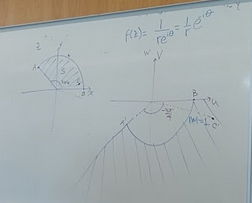
\includegraphics[width=0.4\textwidth]{inversion_dominio.png}
  \end{center}
\end{figure}
\begin{gather}
  \text{Recta }AB:\quad F\left(S \right): \{ \underset{r\in [1,\infty)}{\left|z \right|}\leq 1, \quad -\frac{3\pi}{4}\leq arg(z)\leq 0 \}
\end{gather}

\textbf{Ejemplo } tenemos $ S: \{ z, \quad 2\leq x\leq 5 \} \quad \text{ó} \quad {z, 2\leq Re\left(z \right)\leq 5} $. Al realizar la inversion: 
\begin{gather}
  F\left(z\right)=\frac{1}{z} = \frac{1}{x+iy }\frac{x-iy }{x-iy } = \frac{x-iy }{x ^2 + y ^2}\\
  U = \frac{x }{x ^2 + y ^2}; \qquad V = \frac{-y }{x ^2 + y ^2}\\
  U = \frac{x_0 }{x_0 ^2 + y ^2 }; \qquad V = \frac{-y }{x_0 ^2+y ^2}
\end{gather}
Ahora hacemos $ U ^2+ V ^2 $
\begin{gather}
   U ^2 + V^2 = \frac{x_0 ^2 + y ^2 }{(x_0 ^2+ y ^2)^2} = \frac{1}{x_0 ^2+ y ^2} \rightarrow U ^2 + V ^2 = \frac{U }{x_0 }
\end{gather}
Podemos observar que esto parece un circulo
\begin{gather}
  U ^2 - \frac{u }{x_0 }+ V ^2 = 0 \\
  \rightarrow U ^2 - \frac{U}{x_0 } + \left(\frac{1}{2x_0 }\right)^2 + V ^2 = \left(\frac{1}{2x_0 }\right) ^2\\
  \rightarrow \left(U- \frac{1}{2x_0 }\right) ^2 + V ^2 = \frac{1}{(2x_0 )^2}
\end{gather}
Mapeamos rectas en circulo
\begin{gather}
  \text{Radio del circulo: } x_0 = 5 \rightarrow R = \frac{1}{10 } = 0.1\\
  x_0=2 \rightarrow R = \frac{1}{2x_0 } = \frac{1}{4} = 0.25
\end{gather}
\begin{figure}[H]
  \begin{center}
    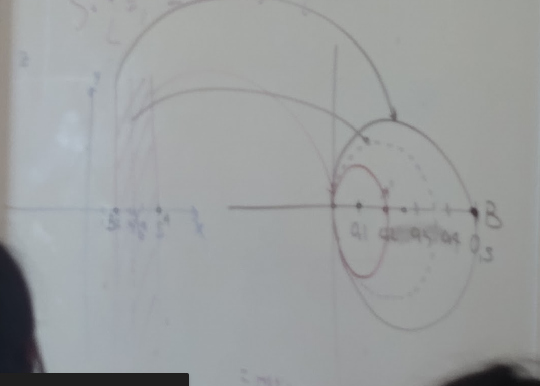
\includegraphics[width=0.4\textwidth]{inversion_rectas.png}
  \end{center}
\end{figure}

\caja{blue}{Tarea}{
  Ver como transforma una franja horizontal.
}


\end{document}
